% -*- root: cuthesis_masters.tex -*-

\section{Approach}
\label{chap3:sec:approach}

\begin{figure}[thb!]
	\centering
	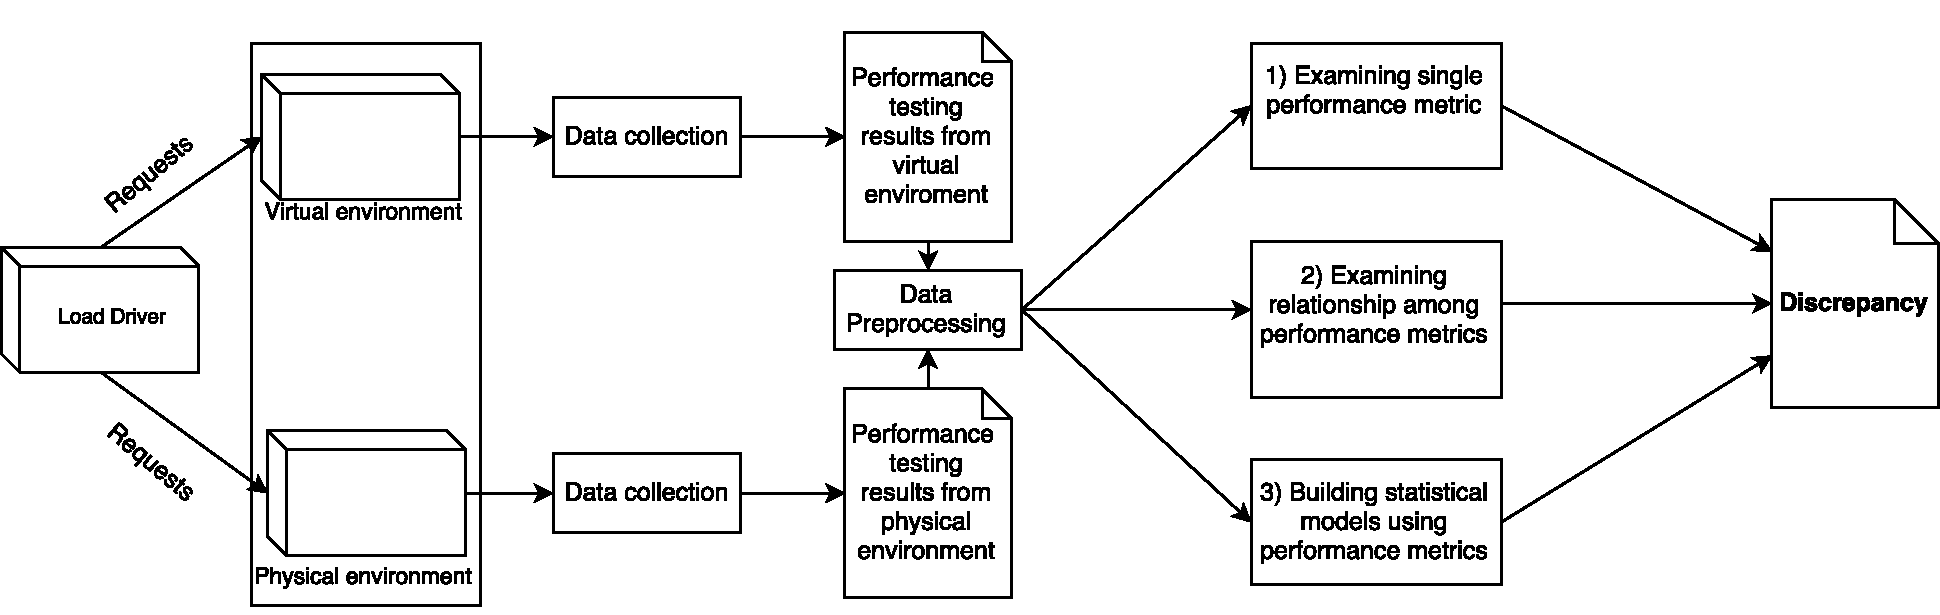
\includegraphics[width=1\textwidth]{figures/overview.pdf}
	\caption{Approach Figure example}
	\label{chap3:fig:approach}
\end{figure}


%\begin{figure}[thb!]
%	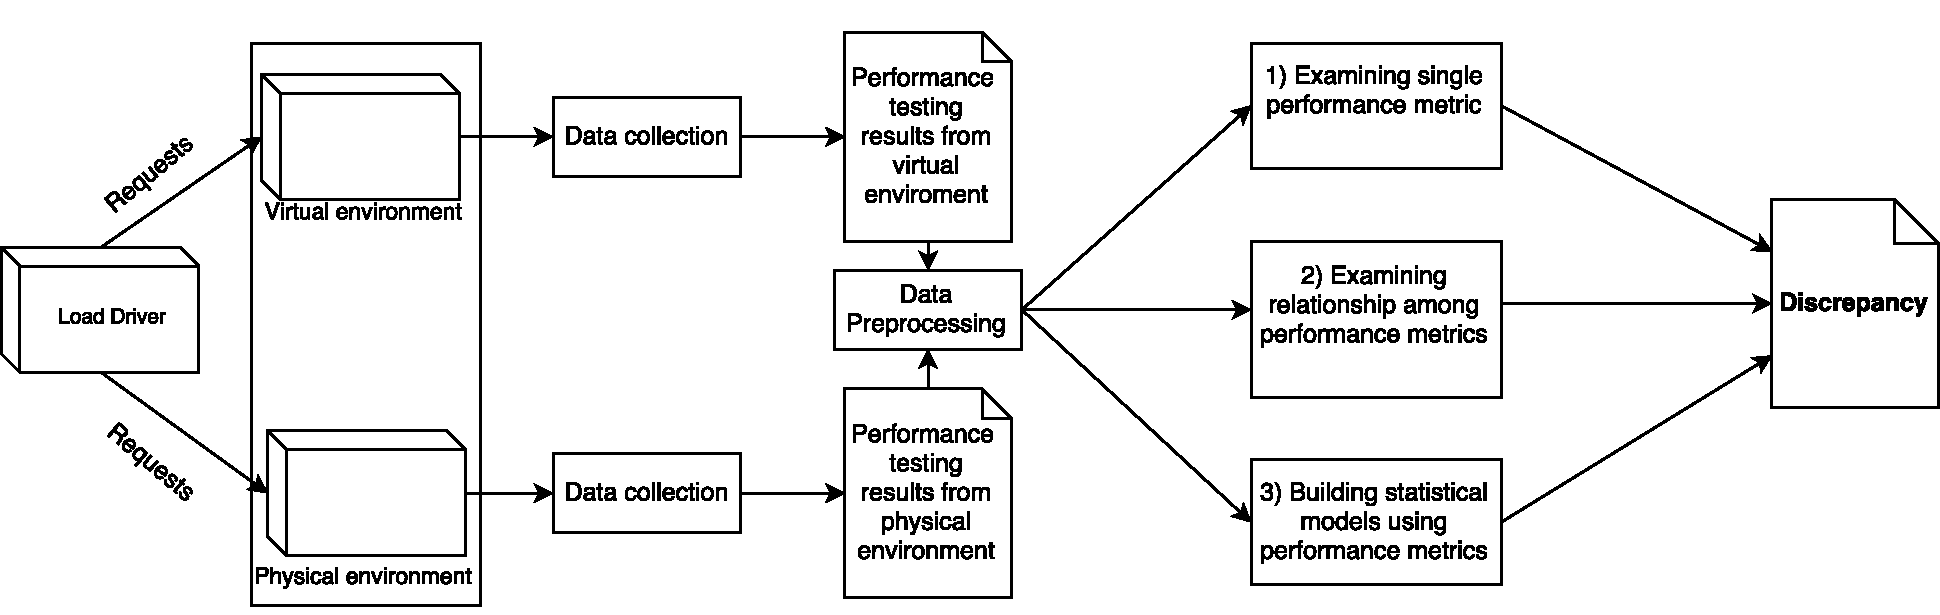
\includegraphics[width=.9\textwidth]{figures/overview}
%	\caption{An overview of our case study setup.}
%	%\captionsetup{justification=centering}
%	\label{fig:Approach}
%\end{figure}

The goal of our case study is to evaluate the discrepancy between performance testing results from virtual and physical environments. We deploy our subject systems in two identical environments(physical and virtual). A load driver is used to exercise our subject systems. After the collection and processing of the performance metrics we analyze and draw conclusions based on: 1) individual performance metrics 2) relationship among performance metrics and 3) statistical models based on the performance metrics. An overview of our case study setup is shown in Figure~\ref{fig:Approach}.


\subsection{Subject Systems}
Dell DVD Store (DS2)~\cite{delldvd} is an online multi-tier e-commerce web application that is widely used in performance testing and prior performance engineering research~\cite{Shang:2015:ADP:2668930.2688052,Nguyen:2012:ADP:2188286.2188344, jackicsm2009}. We deploy DS2 on an Apache (Version 3.0.0) web application server with MySQL 5.6 database server~\cite{mysql}. CloudStore~\cite{cloudstore}, our second subject system is an open source application based on the TPC-W benchmark~\cite{tpcw}. CloudStore is widely used to evaluate the performance of cloud computing infrastructure when hosting web-based software systems and is leveraged in prior research~\cite{tarekmsr16}. We deploy CloudStore on \textit{Apache Tomcat}~\cite{tomcat} (version 7.0.65) with MySQL 5.6 database server~\cite{mysql}. 


\subsection{Environmental Setup}

The performance tests of the two subject systems are conducted on three machines in a lab environment. Each machine has an Intel i5 4690 Haswell Quad-Core 3.50 GHz CPU, with 8 GB of memory, connected to a local gigabyte ethernet. The first machine hosts the web server and application server (Apache and Tomcat). The second machine hosts the MySQL 5.6 database server. The load drivers were deployed on the third machine. We separate the load driver, the web/application server and the database server on different machines in order to mimic real world scenario and avoid interference among these processes. For example, isolating the web and database driver would ensure that the processor is not overused. The operating systems on the three machines are Windows 7. We disable all other processes and unrelated system services to minimize their performance impact. Since our goal is to compare performance metrics in virtual and physical environments, we setup the two different environments, which we detail next.

%was dedicated to the database server, the second machine was dedicated to the web server and the third machine was used to run the load driver.
\noindent \textbf{Virtual environment.} We install one Virtual Box (version 5.0.16) and create only one virtual machine on one physical machine to avoid the interference between virtual machines. For each virtual machine, we allocate two cores and three gigabytes of memory, which is well below capacity to make sure we are topping out and pushing our configuration for unrealistic results. 

%Our virtual setup was identical to our physical setup. The virtual environment was run on the same physical machines with all the resources provided to the host and the same set of aforementioned configuration for the virtual environment. We opted for single tenancy of the guest operating system to avoid any unwanted noise. 

\noindent \textbf{Physical environment.} To make the physical environment similar to the virtual environment, we only enable two cores and 3GB memory for each machine for the physical environment. 

%To make the systems' configuration identical prior to exercising the subject systems, we chose 2 cores and 3GB of memory dedicated to each environment to avoid crashes on the guest operating system in the virtual environment. We also made sure to kill all the processes before we start our performance testing to minimize any discrepancy present.

%\subsection{Exercising the database}
%Following the set up of our subject systems on the respective servers, the systems were exercised with an aid of drivers. These drivers generated multi-type web requests and simulated real-time user behavior depending on the input parameters provided. We ran our performance tests for numerous hours while recording all the performance metrics generated for varying load applied on our software systems.
\subsection{Performance tests}

DS2 is released with a dedicated load driver program that is designed to exercise DS2 for performance testing. We used the load driver to conduct performance testing on DS2. We used Apache JMeter~\cite{apachejmeter} to generate a workload to conduct the performance tests on CloudStore. For both subject systems, the workload of the performance tests is varied periodically in order to avoid bias from a consistent workload. The workload variation was introduced by the number of threads. A higher number of threads represent a higher number of users accessing the system. Each performance test is run after a 15 minute warming up period of the system and lasts for 9 hours. 


%and the last 30 minutes in order to 

%The choice of load was random but consistent between both of the environments. As our study was based on exercising our systems and recording the performance metrics, and not stress testing \cite{stresstesting}, the respected limits were chosen in order to avoid the under-performance of the physical machine and system failure of the virtual machine.


%\subsection{Metrics Collection}
\subsection{Data collection and preprocessing}

\noindent \textbf{Performance metrics.} We used \textit{PerfMon}~\cite{perfmon} to record the values of performance metrics. \textit{PerfMon} is a performance monitoring tool used to observe and record performance metrics such as CPU utilization, memory usage and disk IOs. We record all the available performance metrics that can be monitored on a single process by \emph{PerfMon}.  We recorded the performance metrics of both the processes, web server and the database server, with an interval of 10 seconds. In total, we recorded 44 performance metrics. 

\noindent \textbf{System throughput.} We used the web server access logs from Apache and Tomcat to calculate the throughput of the system by measuring the number of requests per minute. The two data sets were then concatenated and mapped against requests using their respective timestamps.

In order to combine the two datasets of performance metrics and system throughput, and to minimize noise of the performance metric recording, we calculate the mean values of the performance metrics in every minute. Then, we combine the datasets of performance metrics and system throughput based on the time stamp on a per minute basis. A similar approach has been applied to address mining performance metrics challenges~\cite{foo2010mining}.



\section{Case Study Results}
\label{chap3:sec:results}



The goal of our study is to evaluate the discrepancy between performance testing results from virtual and physical environments, particularly considering the impact of discrepancy on the analysis of such results. We do not predict the applications' performance or throughput based on the amount of work done by the underlying architecture or the overhead induced by the virtual environment. Instead, our experiments are set in the context of analyzing performance testing data, based on the related work. Shown in Section~\ref{sec:related}, prior research and practitioners examines performance testing results in three types of approaches: 1) examining individual performance metrics, 2) examining the relationship among performance metrics and 3) building statistical models using performance metrics. Therefore, our experiments focus on examining the discrepancy that may impact three such approaches.



\subsection{Examining individual performance metrics}
\label{sec:individual}
%\emad{Do we want to list a motivation here? Also, do we want to use subsections or RQs to organize the sections.}

\noindent \textbf{Motivation.}
The most intuitive approach of examining performance testing results is to examine individual performance metrics. As shown in Section~\ref{sec:relatedindividual}, prior studies propose different approaches that typically compare the distribution or trend of each performance metric from different tests. Therefore, if the overhead does not impact the shape of the distribution or the trend of the metrics, then the results from heterogeneous environments can be compared.

\noindent \textbf{Approach.} 
After running and collecting the performance metrics, we compare every individual performance metric between the virtual and physical environments. Since the performance tests are conducted in different environments, intuitively the scales of performance metrics are not the same. For example, the virtual environment may have higher CPU usage than the physical environment. Therefore, instead of comparing the values of each performance metric in both environments, we study whether the performance metric follow the same shape of distribution and the same trend in virtual and physical environments. 

First, we plot a quantile-quantile plot (Q-Q plot)~\cite{qqplots} for every performance metric in two environments. A Q-Q plot is a plot of the quantiles of the first data set against the quantiles of the second data set. We also plot a 45-degree reference line on the Q-Q plots. If the performance metrics in both environments follow the same shape of distribution, the points on the Q-Q plots should fall approximately along this reference (i.e., 45-degree) line. A large departure from the reference line indicates that the performance metrics in the virtual and physical environments come from populations with different shapes of distributions, which can lead to different set of conclusions. For example, virtual environment has a CPU's utilization spike at a certain time but the spike is absent in the physical environment. 

Second, to quantitatively measure the discrepancy, we perform a Kolmogorov-Smirnov test~\cite{kstest} between every performance metric in the virtual and physical environments. Since the scales of each performance metric in both environments are not the same, we first normalize the metrics based on their median values and their median absolute deviation: 
\begin{equation}
\label{equ:mad}
M_{normalized}=\frac{M-\tilde{M}}{MAD(M))}		
\end{equation}

where $M_{normalized}$ is the normalized value of the metric, $M$ is the original value of the metric, $\tilde{M}$ is the median value of the metric and $MAD(M)$ is the median absolute deviation of the metric~\cite{walker1929studies}. The Kolmogorov-Smirnov test gives a p-value as the test outcome. A p-value $\leq$ 0.05 means that the result is statistically significant, and we may reject the null hypothesis (i.e., two populations are from the same distribution). By rejecting the null hypothesis, we can accept the alternative hypothesis, which tells us the performance metrics in virtual and physical environments do not have the same distribution. We choose to use the Kolmogorov-Smirnov test since it does not have any assumption on the distribution of the metrics.

Finally, we calculate Spearman's rank correlation between every performance metric in the virtual environment and the corresponding performance metric in the physical environment, in order to assess whether the same performance metrics in two environments follow the same trend during the test. Intuitively, two sets of performance testing results without discrepancy should show similar trend, i.e., when memory keeps increasing in the physical environment (like memory leak), the memory should also increase in the virtual environment. We choose Spearman's rank correlation since it does not have any assumption on the distribution of the metrics. 

\noindent \textbf{Results.}
\textbf{Most performance metrics do not follow the same shape of distribution in virtual and physical environments.} Figure~\ref{fig:qqds2} and \ref{fig:qqcs} show the Q-Q plots by comparing the quantiles of performance metrics from virtual and physical environments. Due to the limited space, we only present Q-Q plot for CPU user time, IO data operations/sec and memory working set for both web sever and database server\footnote{The complete results are shared online at http://das.encs.concordia.ca/wp-content/uploads/2016/04/Arif\_results.zip}. The results show that the lines on the Q-Q plot are not close to the 45-degree reference line. By looking closely on the Q-Q plots we find that the patterns of each performance metric from different subject systems are different. For example, the web CPU user time for DS2 in the virtual environment shows higher values than in the physical environment at the median to high range of the distribution; while the Q-Q plot of CloudStore shows web CPU user time with higher values at the low range of the distribution. In addition, the lines of the Q-Q plots for database memory working set show completely different shapes in DS2 and in CloudStore. The results imply that the discrepancies between virtual and physical environments are present between the subject systems. The impact of the subject systems warrants its own study.

The majority of the performance metrics had statistically significantly different distributions (p-values lower than 0.05 in Kolmogorov-Smirnov tests). Only 13 and 12 metrics (out of 44 for each environment) have p-values higher than 0.05, for DS2 and CloudStore, respectively, showing statistically in-significant difference between the distribution in virtual and physical environments. By looking closely at such metrics, we find that these metrics either do not highly relate to the execution of the subject system (e.g., web server CPU privileged time in DS2), or highly relate to the workload. Since the workload between the two environments are similar, it is expected that the metrics related to the workload follow the same shape of distribution. For example, the I/O operations are highly related with the workload. The metrics related to I/O operations may show statistically in-significant differences between the distributions in the virtual and physical environments (e.g., web server I/O write operations per second in DS2). %\emad{should we list the metrics}


\textbf{Most performance metrics do not have the same trend in virtual and physical environments.} Table~\ref{tab:correlationrq1} shows the Spearman correlation coefficient and corresponding p-value between the selected performance metrics for which we shared the Q-Q plots. We find that for the web server memory working set in CloudStore and the database server memory working set in DS2, there exists strong (0.69) to moderate (0.46) correlation between the virtual and physical environments, respectively. By examining the metrics, we find that both metrics have an increasing trend that may be caused by a memory leak. Such increasing trend may be the cause of the moderate to strong correlation. Instead of showing the selected metrics as the Q-Q plots, Table~\ref{tab:correlationall} shows a summary of the spearman's rank correlation of all the performance metrics. Most of the correlations have an absolute value of 0 to 0.3 (low correlation), or the correlation is not statistically significant (p-val\textgreater0.05).


\noindent\fbox{%
	\parbox{\textwidth}{%
		Performance metrics typically do not follow the same distribution in virtual and physical environments. We conclude that there exists a discrepancy between physical and virtual environment. Practitioners cannot compare individual performance metric with a simple scaling factor applied to the metrics.  
	}%
}


\begin{figure*}[tp]
	\centering
	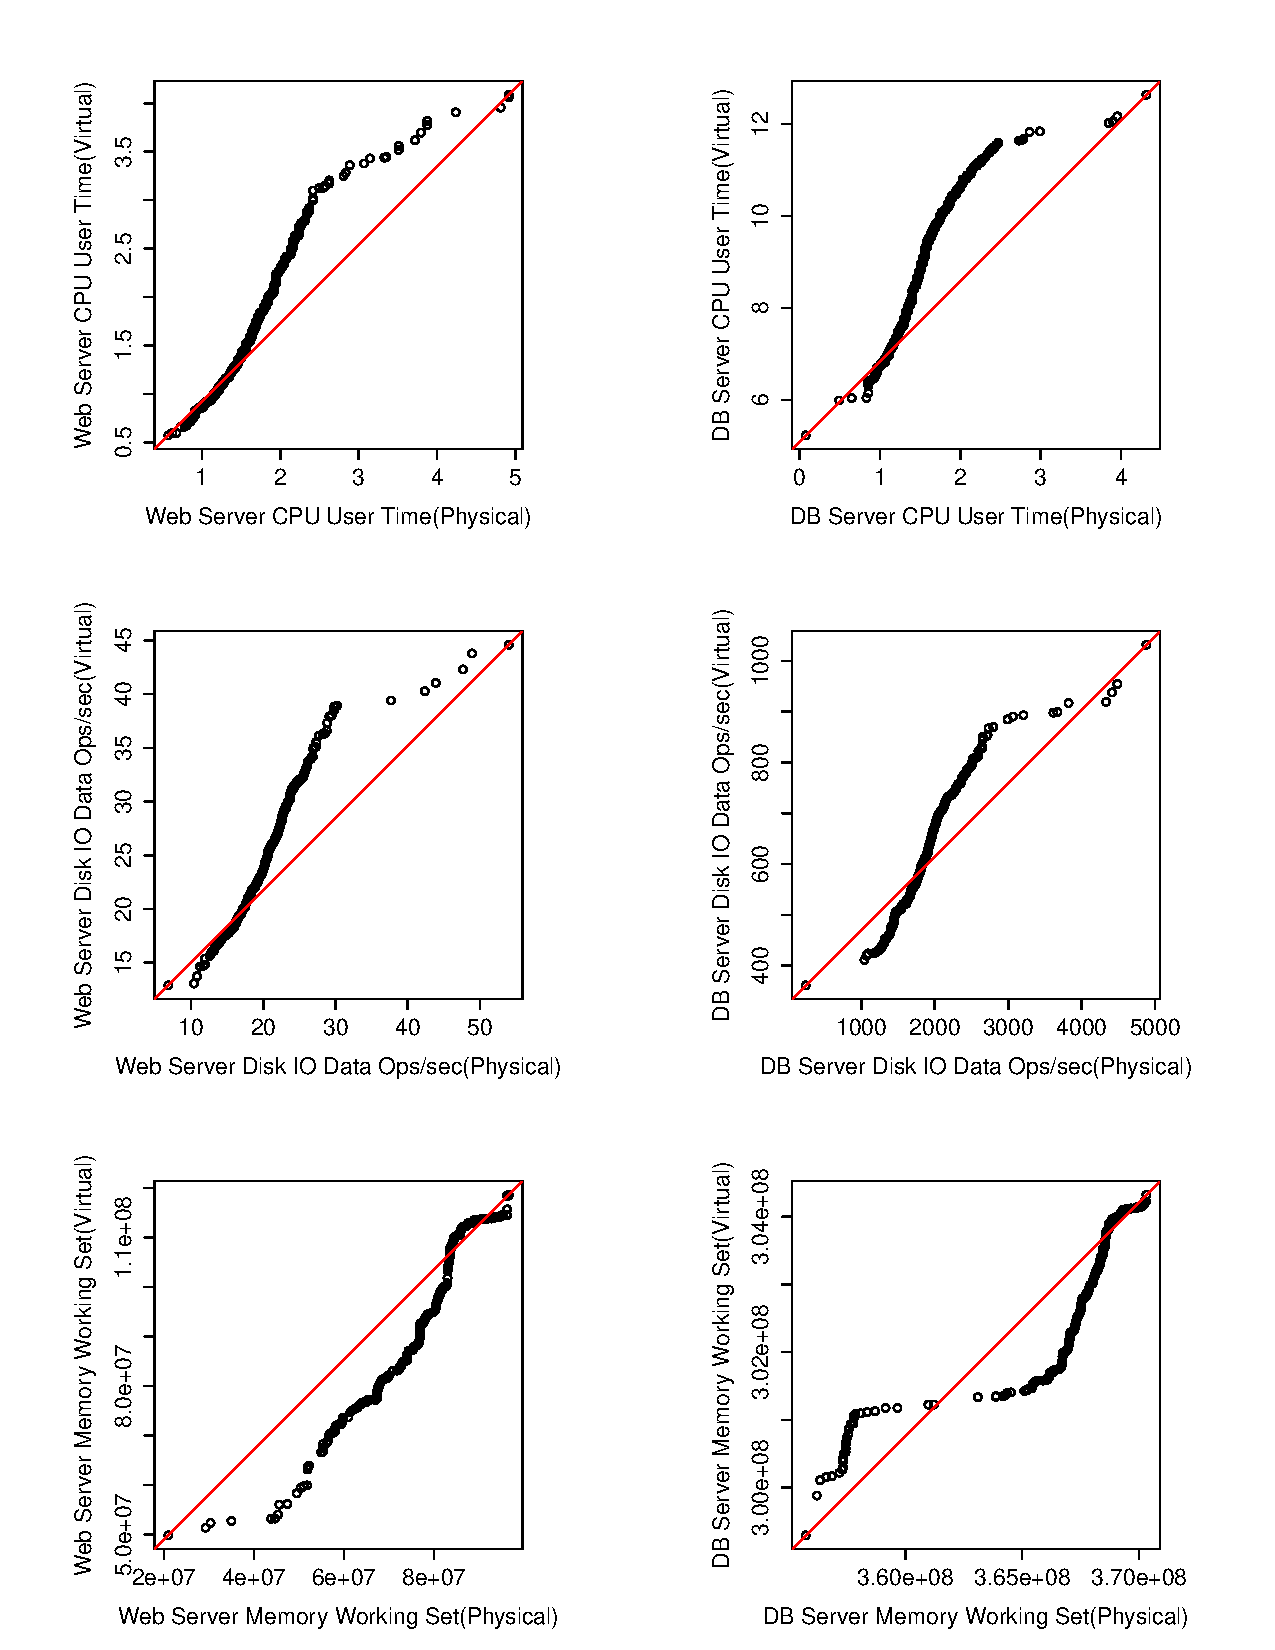
\includegraphics[width=0.9\columnwidth]{figures/ds2_qq_red.pdf}
	\caption{Q-Q plots for DS2.}
	%	\captionsetup{justification=centering}
	\label{fig:qqds2}
\end{figure*}



\begin{figure}[tp]
	\centering
	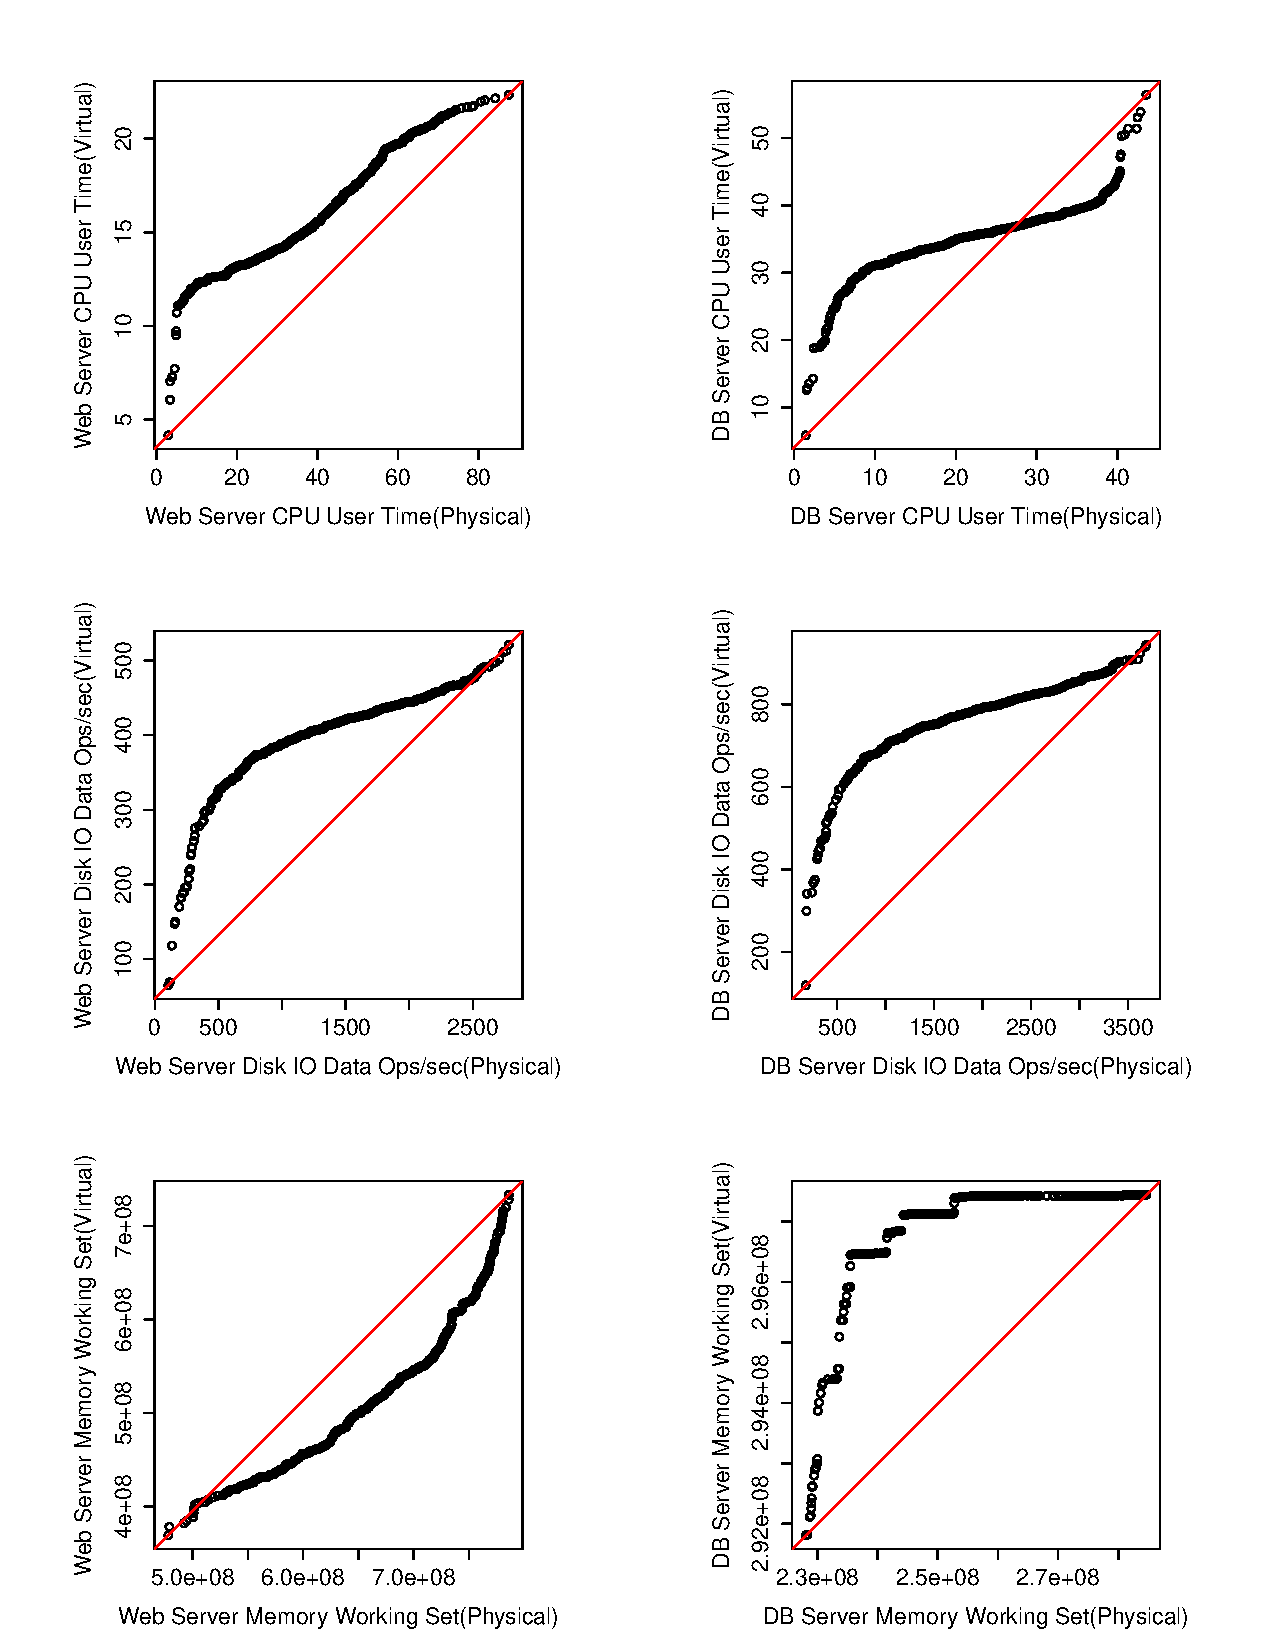
\includegraphics[width=0.9\columnwidth]{figures/cs_523_qq.pdf}
	\caption{Q-Q plots for CloudStore.}
	%	\captionsetup{justification=centering}
	\label{fig:qqcs}
\end{figure}


% Please add the following required packages to your document preamble:
% \usepackage{multirow}
% \usepackage{graphicx}
\begin{table}[tp]
	\centering
	\caption{Spearman's rank correlation coefficients and p-values of the highlighted performance metrics.}
	\label{tab:correlationrq1}
	\begin{tabular}{|c||c|c|c|c|}
		\hline
		\multirow{2}{*}{\textbf{Performance Metrics}} & \multicolumn{2}{c|}{\textbf{DS2}} & \multicolumn{2}{c|}{\textbf{CloudStore}} \\ \cline{2-5} 
		& \textbf{coef.} & \textbf{p-value} & \textbf{coef.} & \textbf{p-value} \\ %\hline
		\midrule 
		\midrule 
		Web Servers' User Times & 0.08 & 0.07 & -0.04 & 0.33 \\ \hline
		DB Servers User Times & -0.05 & 0.30 & 0.10 & 0.02 \\ \hline
		Web Servers' IO Data Ops/sec & 0.25 & 0.00 & 0.13 & 0.00 \\ \hline
		DB Servers' IO Data Ops/sec & -0.14 & 0.00 & 0.13 & 0.00 \\ \hline
		Web Servers' Memory Working Set & 0.22 & 0.00 & 0.69 & 0.00 \\ \hline
		DB Servers' Memory Working Set & 0.46 & 0.00 & -0.16 & 0.00 \\ \hline
	\end{tabular}
\end{table}

\begin{table}[tp]
	\centering
	\caption{Summary of spearman's rank correlation p-values and absolute coefficients of all the performance metrics in DS2 and CloudStore. The numbers in the table are the number of metrics that fall into each category.}
	\label{tab:correlationall}
	\begin{threeparttable}
		
		\begin{tabular}{|c||c|c|c|c|c|}
			\hline
			\multirow{3}{*}{\textbf{System}} & \multirow{3}{*}{\textbf{p-value\textgreater0.05}} & \multicolumn{4}{c|}{\textbf{p-value\textless0.05}} \\ \cline{3-6} 
			&  & \textbf{0.0$\sim$0.3} & \textbf{0.3$\sim$0.5} & \textbf{0.5$\sim$0.7} & \textbf{0.7$\sim$1} \\ %\hline
			\midrule 
			\midrule 
			\textbf{DS2} & 8 & 28 & 4 & 0 & 1 \\ \hline
			\textbf{CloudStore} & 5 & 25 & 4 & 4 & 3 \\ \hline
		\end{tabular}%
		\begin{tablenotes}
			\item Three metrics are constant. Therefore, we do no calculate the correlation on those metrics.
		\end{tablenotes}
	\end{threeparttable}
	
\end{table}



\subsection{Examining the relationship among performance metrics}
\label{sec:relation}
\noindent \textbf{Motivation.}
The relationship between two performance counters may significantly change between two environments, which may be a hint of performance issues or system regressions. For instance, in one release of the system, the CPU may be highly correlated with I/O while (e.g., when I/O is high, CPU is also high); while on a new release of the system, the correlation between CPU and I/O may become low. Such change to the correlation may expose a performance issue (e.g., the high CPU without I/O operation may be due to a performance bug). However, if there is a significant difference in correlations simply due to the platform being used, i.e., virtual vs. physical, then practitioners may need to be warned that a correlation discrepancy may be false. Therefore, we examine whether the relationship among performance metrics has a discrepancy between the virtual and physical environments. 


\noindent \textbf{Approach.} 
We calculate Spearman's rank correlation coefficients among all the metrics from each performance test in each environment. Then we study whether such correlation coefficients are different between the virtual and physical environments. 

First, we compare the changes in correlation between the performance metrics and the system throughput. For example, in one environment, the system throughput may be highly correlated with CPU; while in another environment, such correlation is low. In such a case, we consider there to be a discrepancy in the correlation coefficient between CPU and the system throughput. Second, for every pair of metrics, we calculate the absolute difference between the correlation in two environments. For example, if CPU and Memory have a correlation of $0.3$ in the virtual environment and $0.5$ in the physical environment, we report the absolute difference in correlation as $0.2$ ($|0.3-0.5|$). Since we have 44 metrics in total, we plot a heatmap in order to visualize the 1,936 absolute difference values between every pair of performance metrics. The lighter the color for each block in the heatmap, the larger the absolute difference in correlation between a pair of performance metrics. With the heatmap, we can quickly spot the metrics that have large discrepancy in correlation coefficients. 


\noindent \textbf{Results.}
\noindent \textbf{The correlation between system throughput and performance metrics changes between virtual and physical environments.} Tables~\ref{tab:top10ds2p} and~\ref{tab:top10csp} present the top ten metrics with the highest correlations to system throughput in the physical environment for DS2 and CloudStore, respectively. We chose system throughput to be our touchstone as it was kept identical between the environments.  We find that for these top ten metric sets, the difference in correlation coefficients in virtual and physical environments is up to \textbf{0.78} and the rank changes from \#9 to \#40 in DS2 and \#1 to \#10 in CloudStore.

\noindent \textbf{There exist differences in correlation among the performance metrics from virtual and physical environments.} Figures~\ref{fig:heatmap} and~\ref{fig:heatmap_cs} present the heatmap showing the changes in correlation coefficient among the performance metrics from virtual and physical environments. By looking at the heatmap, we find hotspots (with lighter color), which have larger correlation differences. For the sake of brevity, we do not show all the metric names in our heatmaps. Instead, we enlarge the heatmap by showing one of the hotspots for each subject system in Figures~\ref{fig:heatmap} and~\ref{fig:heatmap_cs}. We find that the hotspots correspond to the changes in correlation among I/O related metrics. Prior research on virtual machines has similar findings about I/O overheads in virtual machines~\cite{menon2005diagnosing,kraft2011io}. In such a situation, when practitioners observe that the relationship between I/O metrics and other metrics change, the change may not indicate a performance regression, but rather the change may be due to the use of a virtual environment.

\noindent\fbox{%
	\parbox{\textwidth}{%
		The correlations between performance metrics and system load may change considerably between virtual and physical environments. The correlation among performance metrics may also change considerably between virtual and physical environments. The correlations that are related with I/O metrics have the largest discrepancy.
	}%
}


\begin{figure*}[tbh!]
	\centering
	{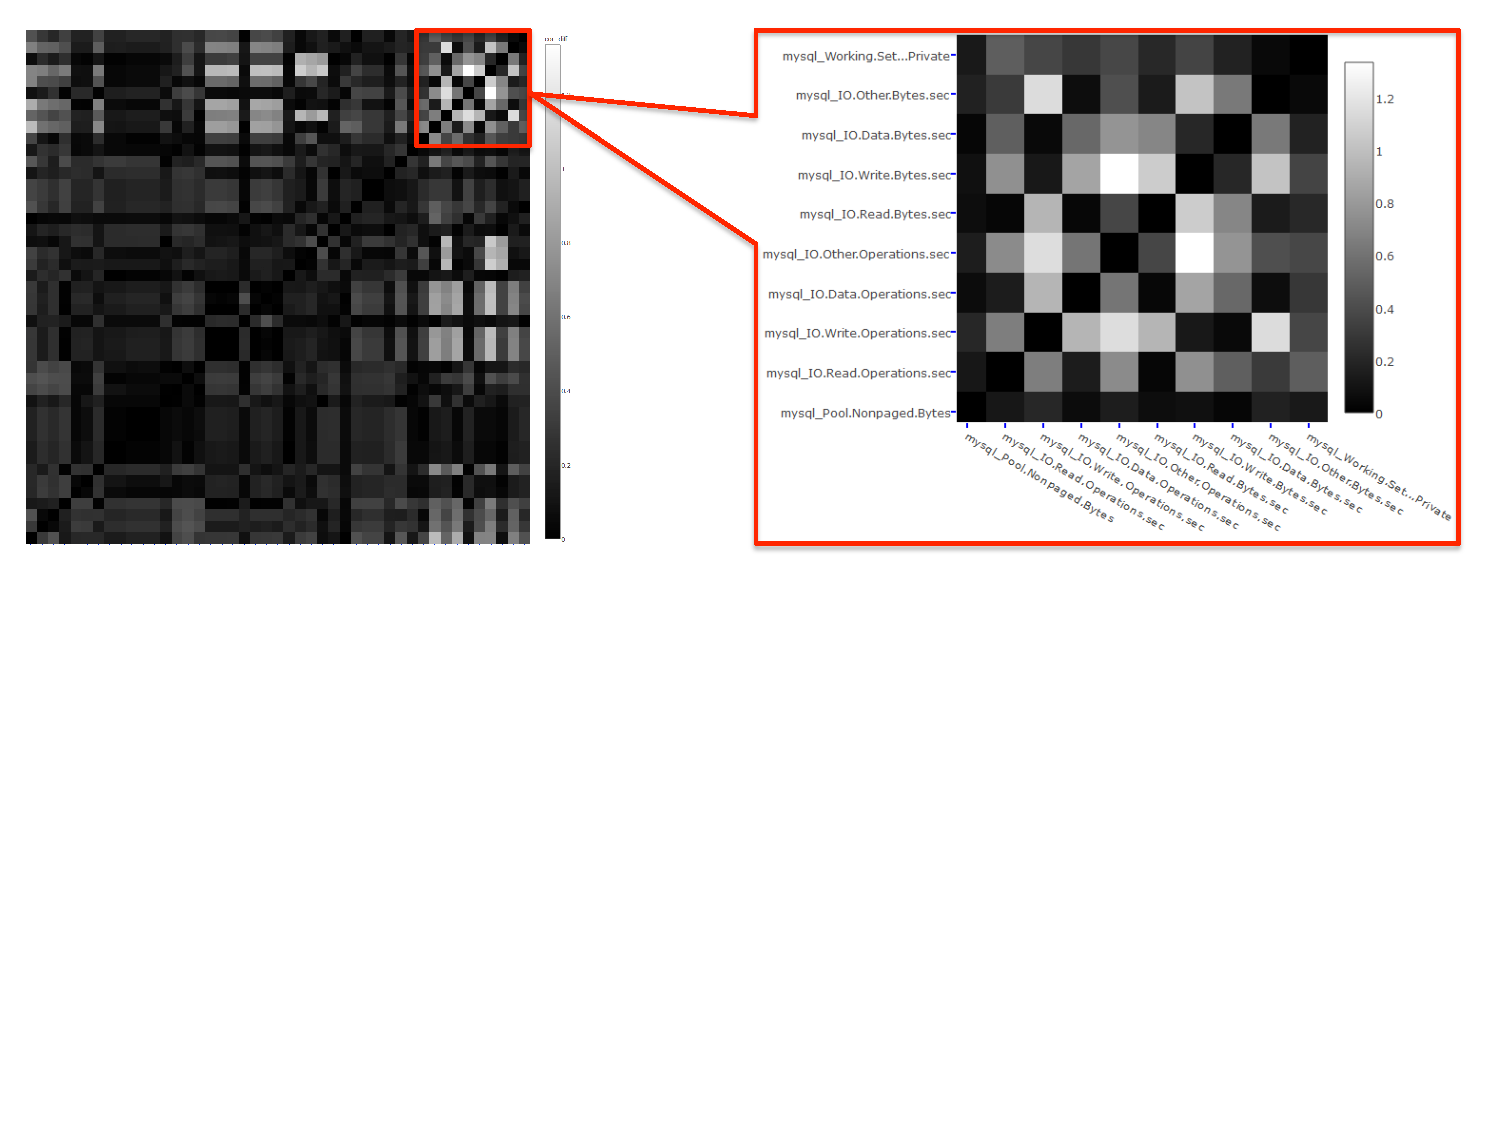
\includegraphics[width=1.0\textwidth]{figures/heat.pdf}}
	\caption{Heatmap of correlation changes for DS2.}
	%\captionsetup{justification=centering}
	\label{fig:heatmap}
\end{figure*}


\begin{figure*}[tbh!]
	\centering
	{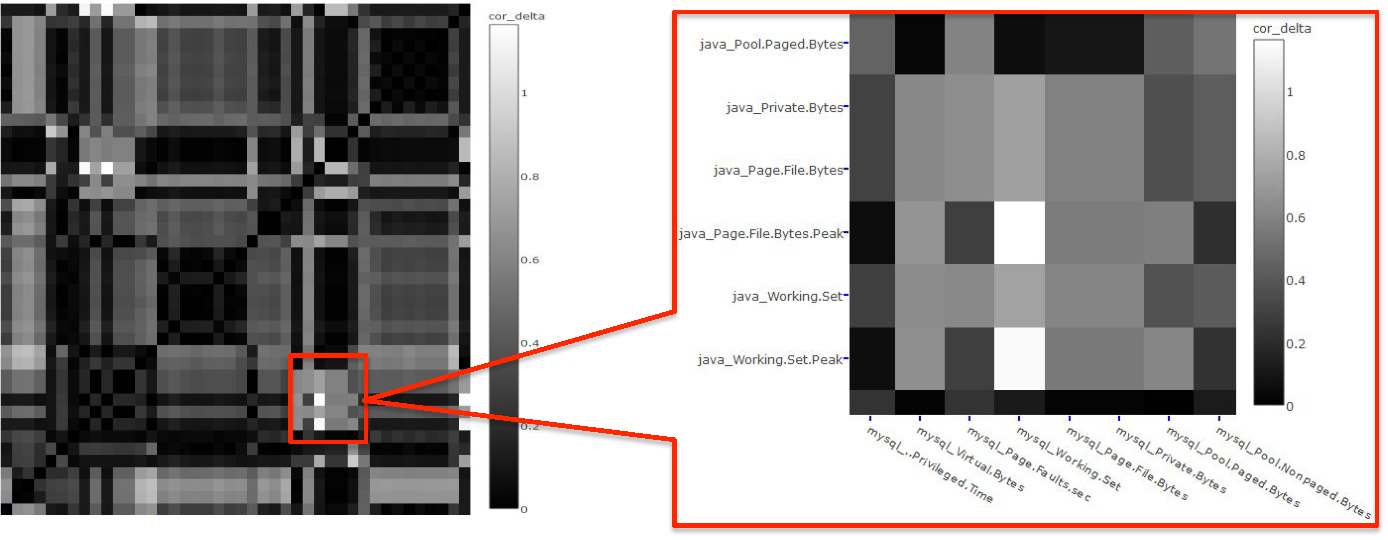
\includegraphics[width=1.0\textwidth]{figures/cloudstore_heat-cropped.pdf}}
	\caption{Heatmap of correlation changes for CloudStore.}
	%\captionsetup{justification=centering}
	\label{fig:heatmap_cs}
\end{figure*}





% Please add the following required packages to your document preamble:
% \usepackage{graphicx}
\begin{table}[tbh]
	\centering
	\caption{Top ten metrics with highest correlation coefficient to system throughput in the physical environment for DS2. }
	\label{tab:top10ds2p}
	\begin{threeparttable}
		
		\begin{tabular}{|c||c|c|c|c|}
			\hline
			\textbf{Rank} & \textbf{Performance } & \textbf{Coef. } & \textbf{Coef. } & \textbf{Rank in} \\ %\hline
			& \textbf{ Metrics} & \textbf{PE} & \textbf{VE} & \textbf{VE} \\ %\hline
			\midrule
			\midrule
			1 & Web IO Other Ops/sec & 0.91 & 0.62 & 10 \\ \hline
			2 & Web IO Other Bytes/sec & 0.91 & 0.62 & 12 \\ \hline
			3 & Web IO Write Ops/sec & 0.91 & 0.63 & 9 \\ \hline
			4 & Web IO Data Ops/sec & 0.91 & 0.63 & 8 \\ \hline
			5 & Web IO Write Bytes/sec & 0.90 & 0.62 & 11 \\ \hline
			6 & Web IO Data Bytes/sec & 0.90 & 0.61 & 13 \\ \hline
			7 & DB IO Other Ops/sec & 0.84 & 0.75 & 3 \\ \hline
			8 & DB IO Data Ops/sec & 0.83 & 0.07 & 41 \\ \hline
			9 & DB IO Other Bytes/sec & 0.83 & 0.15 & 40 \\ \hline
			10 & DB IO Read Ops/sec & 0.82 & 0.15 & 39 \\ \hline
		\end{tabular}%
		\begin{tablenotes}
			\item PE in the table is short for physical environment; while VE is short for virtual environment.
		\end{tablenotes}
	\end{threeparttable}
	
	
\end{table}

\begin{table}[tbh]
	\centering
	\caption{Top ten metrics with highest correlation coefficient to system throughput in the physical environment for CloudStore}
	\label{tab:top10csp}
	\begin{threeparttable}
		
		\begin{tabular}{|c||c|c|c|c|}
			\hline
			\textbf{Rank} & \textbf{Performance } & \textbf{Coef. } & \textbf{Coef. } & \textbf{Rank in} \\ %\hline
			& \textbf{ Metrics} & \textbf{PE} & \textbf{VE} & \textbf{VE} \\ %\hline
			\midrule
			\midrule
			1 & DB Server IO Other Bytes/sec & 0.98 & 0.73 & 10 \\ \hline
			2 & DB Server IO Read Ops/sec & 0.98 & 0.84 & 7 \\ \hline
			3 & DB Server IO Read Bytes/sec & 0.98 & 0.93 & 5 \\ \hline
			4 & DB Server IO Write Ops/sec & 0.98 & 0.97 & 2 \\ \hline
			5 & DB Server IO Data Ops/sec & 0.98 & 0.92 & 6 \\ \hline
			6 & DB Server IO Data Bytes/sec & 0.98 & 0.96 & 4 \\ \hline
			7 & DB Server IO Write Bytes/sec & 0.98 & 0.96 & 3 \\ \hline
			8 & Web Server IO Other Bytes/sec & 0.98 & 0.68 & 16 \\ \hline
			9 & DB Server IO Other Ops/sec & 0.98 & 0.98 & 1 \\ \hline
			10 & Web Server IO Other Ops/sec & 0.98 & 0.70 & 14 \\ \hline
		\end{tabular}%
		\begin{tablenotes}
			\item PE in the table is short for physical environment; while VE is short for virtual environment.
		\end{tablenotes}
	\end{threeparttable}
	
	
\end{table}


%\begin{table*}[tbh]
%	\centering
%	\caption{CloudStore: Top 10 highly correlated metrics with load (Physical Server)}
%	\label{my-label}
%	\resizebox{\textwidth}{!}{%
%		\begin{tabular}{|c||c|c|c|c|}
%			\hline
%			\textbf{Rank} & \textbf{Performance Metrics} & \textbf{Cor in Physical Environment} & \textbf{Cor in Virtual Environment} & \textbf{Rank in Virtual Environment} \\ %\hline
%			\midrule
%			\midrule
%			1 & DB Server IO Other Bytes/sec & 0.98 & 0.73 & 10 \\ \hline
%			2 & DB Server IO Read Ops/sec & 0.98 & 0.84 & 7 \\ \hline
%			3 & DB Server IO Read Bytes/sec & 0.98 & 0.93 & 5 \\ \hline
%			4 & DB Server IO Write Ops/sec & 0.98 & 0.97 & 2 \\ \hline
%			5 & DB Server IO Data Ops/sec & 0.98 & 0.92 & 6 \\ \hline
%			6 & DB Server IO Data Bytes/sec & 0.98 & 0.96 & 4 \\ \hline
%			7 & DB Server IO Write Bytes/sec & 0.98 & 0.96 & 3 \\ \hline
%			8 & Web Server IO Other Bytes/sec & 0.98 & 0.68 & 16 \\ \hline
%			9 & DB Server IO Other Ops/sec & 0.98 & 0.98 & 1 \\ \hline
%			10 & Web Server IO Other Ops/sec & 0.98 & 0.70 & 14 \\ \hline
%		\end{tabular}%
%	}
%\end{table*}


%\begin{table*}[tbh]
%	\centering
%	\caption{CloudStore: Top 10 highly correlated metrics with load (Virtual Server)}
%	\label{my-label}
%	\resizebox{\textwidth}{!}{%
%		\begin{tabular}{|c||c|c|c|c|}
%			\hline
%			\textbf{Rank} & \textbf{Performance Metrics} & \textbf{Cor in Virtual Environment} & \textbf{Cor in Physical Environment} & \textbf{Rank in Physical Environment} \\ %\hline
%			\midrule
%	     	\midrule
%			1 & DB Server IO Other Ops/sec & 0.98 & 0.98 & 9 \\ \hline
%			2 & DB Server IO Write Ops/sec & 0.97 & 0.98 & 4 \\ \hline
%			3 & DB Server IO Write Bytes/Sec & 0.96 & 0.98 & 7 \\ \hline
%			4 & DB Server IO Data Bytes/sec & 0.96 & 0.98 & 6 \\ \hline
%			5 & DB Server IO Read Bytes/sec & 0.93 & 0.98 & 3 \\ \hline
%			6 & DB Server IO Data Ops/sec & 0.92 & 0.98 & 5 \\ \hline
%			7 & DB Server IO Read Ops/sec & 0.83 & 0.98 & 2 \\ \hline
%			8 & DB Server User Time & 0.78 & 0.89 & 22 \\ \hline
%			9 & DB Server Processor Time & 0.76 & 0.91 & 21 \\ \hline
%			10 & DB Server IO Other Bytes/sec & 0.72 & 0.97 & 1 \\ \hline
%		\end{tabular}%
%	}
%\end{table*}

\subsection{Building statistical models using performance metrics}
\label{sec:model}
%\textbf{Motivation}: As discussed in earlier work \cite{Shang:2015:ADP:2668930.2688052} \cite{Nguyen:2012:ADP:2188286.2188344}, performance tests require a large dedication of resources as it is carried out just before the system is on the brink of deployment. This gives insufficient time to the performance engineers, leaving them with minimal resources. As a result they leverage on the performance assurance activities carried out in the virtual environment. The motivation behind this research question is to investigate whether the performance models generated from one environment can be applied and held representatives of the other. In essence, this will help the practitioners conclude the reliability of the performance activities carried out in the virtual environment. 
% In practice, this may or may not be appropriate to assume. This also spawns the concept of including the entire set of performance metrics for analysis, which is slipshod and ineffectual. 

\noindent \textbf{Motivation.}
As discussed in the last step (c.f., Section~\ref{sec:relation}), the relationship among performance metrics is critical for examining performance testing results (c.f., Section~\ref{sec:relatedrelation}). However, thus far we have only examined the relationships between two performance metrics. In order to capture the relationship among a large number of performance metrics, more complex modeling techniques are needed. More importantly, some performance metrics do not have any impact with system performance, which are still examined. For example, for a software system that is CPU intensive, I/O operations may be irrelevant. Such performance metrics may expose large discrepancies between virtual and physical environments, but they do not impact the examination of performance testing results. To address the above issues, modeling techniques are proposed to examine performance testing results (c.f., Section~\ref{sec:relatedmodel}). In this step, we examine whether the modeling among performance metrics has a discrepancy between the virtual and physical environments and whether we can minimize such discrepancy between performance models.


\noindent \textbf{Approach. }

%\emad{we should really add a reason as to why we are doing this}
We follow a model building approach that is similar to the approach from prior research~\cite{Shang:2015:ADP:2668930.2688052,Cohen:2005:CIC:1095810.1095821,xiong2013vperfguard}. We first build statistical models using performance metrics from one environment, then we test the accuracy of our performance model with the metric values from the same environment and also from a different environment. For example, if the model was built in a physical environment it was tested in both, physical and virtual environment.

\subsubsection{B-1: Reducing counters}

Mathematically, performance metrics that show little or no variation do not contribute to the statistical models hence we first remove performance metrics that have constant values in the test results. We then perform a correlation analysis on the performance metrics. We used the Spearman's rank correlation coefficient among all performance metrics from one environment. We find the pair of performance metrics that have a correlation higher than 0.75 \cite{Syer2016}. From these two performance metrics, we remove the metric that has a higher average correlation with all other metrics. We repeat this step until there exists no correlation higher than 0.75.

We then perform redundancy analysis on the performance metrics. The redundancy analysis would consider a performance metric redundant if it can be predicted from a combination of other metrics~\cite{harrell2001regression}. We use each performance metric as a dependent variable and use the rest of the metrics as independent variables to build a regression model. We calculate the $R^2$ of each model and if the $R^2$ is larger than a threshold (0.9)\cite{Syer2016}, the current dependent variable (i.e., performance metric) is considered redundant. We then remove the performance metric with the highest $R^2$ and repeat the process until no performance metric can be predicted with $R^2$ higher than the threshold. For example, if CPU can be linearly modeled by the rest of the performance metrics with $R^2\textgreater0.9$, we remove the metric for CPU.

Not all the metrics in the model are statistically significant. Therefore in this step, we only keep the metrics that have a statistically significant contribution to the model. We leverage the \textit{stepwise} function that adds the independent variables one by one to the model to exclude any metrics that are not contributing to the model~\cite{RInAction}. 

\subsubsection{B-2: Building statistical models}

In the second step, we build a regression model~\cite{freedman2009statistical} using the performance metrics that are left after the reduction and removal of statistically insignificant metrics in the previous step as independent variables and use the system throughput as our dependent variable. Similar models have been built in prior research~\cite{Cohen:2005:CIC:1095810.1095821,xiong2013vperfguard}.

%\subsubsection{B-3: Finalizing statistical models}
After removing all the insignificant metrics, we have all the metrics that significantly contribute to the model. We use these metrics as independent variables to build the final model.

\subsubsection{V-1: Validating model fit}

Before we validate the model with internal and external data, we first examine how good the model fit is. If the model has a poor fit to the data, then our findings from the model may be biased by the noise from the poor model quality. We calculate the $R^2$ of each model to measure fit. If the model perfectly fits the data, the $R^2$ of the model is 1, while a zero $R^2$ value indicates that the model does not explain the variability of the response data. We also would like to estimate the impact that each independent variable has on the model fit. We follow a ``drop one'' approach~\cite{Chambers1990}, which measures the impact of an independent variable on a model by measuring the difference in the performance of models built using: (1) all independent variables (the full model), and (2) all independent variables except for the one under test (the dropped model). A Wald statistic is reported by comparing the performance of these two models ~\cite{harrell2001regression}. A larger Wald statistic indicates that an independent variable has a larger impact on the model's performance, i.e., model fit. A similar approach has been leveraged by prior research in~\cite{mcintosh2015emse}. We then rank the independent variables by their impact on model fit. 


%After removing any outliers for both of our subject systems, we built our GLM, initially, using all the physical server's metrics. We trained and tested our model on the same server i.e. physical. We then reduced our model, iteratively, using only the metrics that our contributing the most to the model. This was achieved using R's \textit{stepwise} function. The \textit{stepwise} function adds the independent variables one by one to the model to exclude any metrics that not contributing to the model \cite{RInAction}. Once the metrics were automatically selected out on the physical server, we used R's \textit{ANOVA}, or \textit{analysis of deviance} to rank the metrics according to their deviance value. Higher the deviance value for a given performance metric in the model, higher the contribution of the performance metric to the model. This approach was similarly applied to the set of metrics from the virtual server to build a generalized linear model. R's \textit{deviancepercentage} was used to determine the explanatory part or fit of our model. It is used to calculate the percentage of deviance for a given GLM model.

\subsubsection{V-2: Internal validation}

We validate our models with the performance testing data that is from the same environment. We leverage a standard 10-fold cross validation process, which starts by partitioning the performance data to 10 partitions. We take one partition (fold) at a time as the test set, and train on the remaining nine partitions~\cite{10foldcross,kohavi1995study}, similar to prior research~\cite{haroon}. For every data point in the testing data, we calculate the absolute percentage error. For example, for a data point with a throughput value of 100 requests per minute, if our predicted value is 110 requests per minute, the absolute percentage error is $0.1$ ($\frac{|110-100|}{100}$). After the ten-fold cross validation, we have a distribution of absolute percentage error (\textit{MAPE}) for all the data records.

%We partitioned our results into two segments; the explanatory and the predictive part for our models, trailed by applying our model to predict load cross-environments. The explanatory part calculates the percentage of deviance explained by our models i.e. the fit of the model while the predictive part explains the error percentage between the actual and predicted load values. Both of these parts were addressed by building generalized linear models that only incorporated the metrics which were selected via R \textit{stepwise stepwise} or commonly knows as \textit{stepwise} function, from the complete set of metrics from the dataset.


\subsubsection{V-3: External validation}
To evaluate whether the model built using performance testing data in one environment (e.g., virtual environment) can apply to another environment (e.g., physical environment), we test the model using the data from the other environment.

Since the performance testing data is generated from different environments, directly applying the data on the model would intuitively generate large amounts of error. We adopt two approaches in order to normalize the data in different environments: (1) \textbf{Normalization by deviance.} The first approach we use is the same when we compare the distribution of each individual performance counter shown in Equation~\ref{equ:mad} from Section~\ref{sec:individual} by calculating the relative deviance of a metric value from its median value. (2) \textbf{Normalization by load.} The second approach that we adopt is an approach that is proposed by Nguyen \textit{et al.}~\cite{Nguyen:2012:ADP:2188286.2188344}. The approach uses the load of the system to normalize the performance metric values across different environments. As there are varying inputs for the performance tests that we carried out, normalization by load helps in normalizing the multi-modal distribution that might be because of the trivial tasks like background processes(bookkeeping).

%We addressed the presence of a high percentage error by adjusting our virtual environment's metrics to the phsyiscal environment according to the following equation:
%As explained in RQ1, we perceived that our distributions generated by the performance metrics in our environments are not the same. We used R's \textit{predict} to predict our desired set of load, based on the training and testing mentioned in the previous subsections. \textcolor{red}{we used 1-fold cross validation here, necesaary to mention?}


To normalize our metrics, we first build a linear regression model with the one metric as an independent variable and the throughput of the system as the dependent variable. With the linear regression model in one environment, the metric values can be represented by the system throughput. Then we normalize the metric value by the linear regression from the other environment. The details of the metric transformation are shown as follows:

\begin{equation*}
throughput_{p}= \alpha_{p} \times M_{p} + \beta_{p}
\end{equation*}
\vspace{-0.4cm}
\begin{equation*}
throughput_{v}= \alpha_{v} \times M_{v} + \beta_{v}
\end{equation*}
\vspace{-0.4cm}
\begin{equation*}
M_{normalized} = \frac{(\alpha_{v} \times M_{v})+\beta_{v}-\beta_{p}}{\alpha_{p}}
\end{equation*}
where $throughput_{p}$ and $throughput_{v}$ are the system throughput in the physical and virtual environment, respectively. $M_{p}$ and $M_{v}$ are the performance metrics from both environments, while $M_{normalized}$ is the metric after normalization. $\alpha$ and $\beta$ are the coefficient and intercept values for the linear regression models. After normalization, we calculate the absolute percentage error for every data record in the testing data.


%The selected counter was chosen on the basis of counters selected by \textit{stepwise}, trained in virtual and tested in physical environment. For every GLM there exists an intercept and a gradient value. We used the aforementioned values and applied them to the metric from the virtual environment as explained by equation 1.
%We also assumed that for each of the metric there will be a gradient and intercept value.




\subsubsection{Identifying model discrepancy}
In order to identify the discrepancy between the models built using data from the virtual and physical environments, we compare the two distributions of absolute percentage error based on our internal and external validation. If the two distributions are significantly different (e.g., the absolute percentage error from internal validation is much lower than that from external validation), the two models are considered to have a discrepancy. To be more concrete, in total for each subject system, we ended up with four distributions of absolute percentage error: 1) modeling using the virtual environment and testing internally (on data from the virtual environment), 2) modeling using the virtual environment and testing externally (on data from the physical environment), 3) modeling using the physical environment and testing internally (on data from the physical environment), 4) modeling using the physical environment and testing externally (on data from the virtual environment). We compare distributions 1) and 2) and we compare distributions 3) and 4). Since normalization based on deviance will change the metrics values to be negative when the metric value is lower than median, such negative values cannot be used to calculate absolute percentage error. We perform a min-max normalization on the metric values before calculating the absolute percentage error. In addition, if the observed throughput value after normalization is zero (when the observed throughput value is the minimum value of both the observed and predicted throughput values), we cannot calculate the absolute percentage error for that particular data record. Therefore, we remove the data record if the throughput value after normalization is zero. In our case study, we only removed one data record when performing external validation with the model built in the physical environment. 


\noindent \textbf{Results.}

\noindent \textbf{The statistically significant performance metrics leveraged by the models in virtual and physical environments are not the same.} Tables~\ref{tab:modelsummaryds2} and \ref{tab:modelsummarycs} show the summary of the statistical models built for the virtual and physical environments for the two subject systems. We find that all the models have good model fit (66.9\% to 94.6\%). However, some statistically significant independent variables in one model do not appear in the other model. For example, Web Server Virtual Bytes ranks \#4 for the model built from the physical environment data of CloudStore, while the metric is not significant in the model built from the virtual environment data. In fact, none of the significant variables in the model built from the virtual environment are related to the web server's memory (see Table~\ref{tab:modelsummarycs}). We do observe some performance metrics that are significant in both models even with the same ranking. For example, Web Server IO Other Bytes/sec is the \#1 significant metric for both models built from the virtual and physical environment data of DS2 (see Table~\ref{tab:modelsummaryds2}). 

\noindent \textbf{The prediction error illustrates discrepancies between models built in virtual and physical environments.} Although the significant independent variables in the models built by the performance testing results in the virtual and physical environments are different, the model may have similar prediction results due to correlations between metrics. However, we find that the external prediction errors are higher than internal prediction errors for all four models from the virtual and physical environments for the two subject systems. In particular, Table~\ref{tab:errors} shows the prediction errors using normalization based on load is always higher than that of the internal validation. For example, the median absolute percentage error for CloudStore using normalization by load is 632\% and 483\% for the models built in the physical environment and virtual environment, respectively; while the median absolute percentage error in interval validation is only 2\% and 10\% for the models built in the physical and virtual environments, respectively. However, in some cases, the normalization by deviance can produce low absolute percentage error in external validation. For example, the median absolute percentage error for CloudStore can be reduced to 9\% using normalization by deviance. 

One possible reason is that the normalization based on load performs better, even though it is shown to be effective in prior research~\cite{Nguyen:2012:ADP:2188286.2188344}, assumes a linear relationship between the performance metric and the system load. However, such an assumption may not be true in some performance testing results. For example, Table~\ref{tab:top10ds2p} shows that some I/O related metrics do have low correlation with the system load in virtual environments. On the other hand, the normalization based on deviance shows much lower prediction error. We think the reason is that the virtual environments may introduce metric values with high variance. Normalizing based on the deviance controls such variance, leading to lower prediction errors.

%\ian{todo} Tables 7-10 show the results of our approach. In Table 7, for our subject system DS2, we see that the statistically significant metrics for the GLM from both of our environments are different. The significant of the performance metrics in an GLM is environment dependent. Due to automatic selection of metrics we see a high fit and lower \textit{MAPE} values for our environments. Table 8 shows us the results when the model from the virtual was applied to predict load for the physical server and vice-versa. We observe a an immensely high \textit{MAPE} value for the former while physical-virtual prediction is almost 50\%. This means that the predicted and actual values of the workload have a mean absolute error percentage of almost 50\%. When the same set of metrics from the virtual environment were scaled the MAPE value for DS2 reduces drastically.




%We obtained the former equations with the models by training and testing on the respective environments. These equations are derived from the previous work of \cite{Nguyen:2012:ADP:2188286.2188344} Once, the model was constructed we extracted the \(\alpha\) and \(\beta\) values from each model and applied them to scale the virtual environment's metrics accordingly. Equation (1) shows the derived equation through which we scaled the metrics during the process of scaling the counters. 


%As shown in Table 3, we concluded that most of the contributions to our models are by \textit{DISC IO} and the \textit{CPU}. Inclusion of the aforementioned set of performance metrics gave us a fit percentage closer to the models which included all of the performance metrics. Additionally, the models that were based on the statistically significant metrics ranked by the other environment showed a MAPE value of no more than 7\%. This helped us conclude the metrics that are contributing the most between are environments are overlapping.  
%The unscaled transfer of metrics generated a \textit{MAPE} value \textbf{40\%} more than that of scaled counters. Our approach successfully identified that the performance metrics generated in the virtual environment can not be taken as the exact reflection of the performance of the system in the physical environment. We also deduced the diversity in environment does impact the regression models and the performance assurance activities. One of the solution to counters this is scaling, however, the error still remains relatively high as shown in Table 2.

%\afterpage{%
%    \clearpage% Flush earlier floats (otherwise order might not be correct)
%    \thispagestyle{empty}% empty page style (?)
%    \begin{landscape}% Landscape page
%        \centering % Center table
%        \begin{tabular}{llll}
%          \begin{table}[thb!]
%    \begin{center}
%    \caption{Results}
%    \label{tab:project_results}
%            \begin{tabular}{c||cccc}
%            \toprule
%            \textbf{Training-Testing}   & \textbf{Physical - Physical} & \textbf{Physical - Virtual} & \textbf{Virtual - Virtual} & \textbf{Virtual - Physical} \\  
%            \midrule 
%            \textbf{Ranking}     &       1. IO Read Bytes/sec & 1.IO Read Bytes/sec & 1.User Time  & 1.IO Read Operations/sec \\
%             &                               2. IO Data Operations/sec & 2. IO Data Operations/sec & 2. IO Read Bytes/sec & 2. IO Read Operations/sec \\
%             & 3.IO Read Operations/sec & 3.IO Other Bytes/sec & 3. IO Data Operations/sec & 3. IO Other Bytes/sec \\
%             & 4. IO Other Bytes/sec & 4. IO Read Operations/sec & 4. IO Other Bytes/sec & 4. IO Write Bytes/sec\\
%             & 5.IO Data Bytes/sec & & 5.Elapsed Time &\\
%             & 6.Page Faults/sec & & 6.IO Read Operations/sec &\\
%             & & & 7. Thread Count &\\
%             & & & 8. IO Write Bytes/sec &\\
%             & & & 9.IO Write Operations/sec &\\
%             & & & 10. Working Set &\\
%             \midrule
%             \textbf{Fit} & All metrics: 64.1\% & All metrics: 81\% & All metrics: 81\% & All metrics: 63.4\%\\
%             & Statistically Significant Metrics: 63.5\% & Statistically Significant Metrics: 81\% & Statistically Significant Metrics: 81\% & Statistically Significant Metrics: 63.2\% \\
%             \midrule
%             \textbf{MAPE} & 6.17\% & 3.81\% & 3.89\% & 6.14\% \\
%            \bottomrule             
%        \end{tabular}
%    \end{center}
%\end{table}
%\\
%        \end{tabular}
%        \captionof{table}{Table caption}% Add 'table' caption
%    \end{landscape}
%    \clearpage% Flush page
%}

%\end{description}

%%\begin{landscape}
%	\begin{table}[tbh]
%		\centering
%			\caption{DS2: Ranking of Performance Counters and Prediction errors}
%			\label{tab:resultRQ1}
%			\resizebox{\columnwidth}{!}{%
%			\begin{tabular}{c||cc}
%				\toprule
%				\textbf{Training-Testing} & \textbf{Physical - Physical} & \textbf{Virtual - Virtual} \\  
%				\midrule 
%				\textbf{Ranking}     & 1. Web Server Privileged Time & 1. Web Server IO Other Bytes/sec \\
%				\\
%				& 2. Database Server User Time & 2. Web Server Page Faults/sec \\
%				\\
%				& 3. Database Server IO Read Bytes/sec & 3.Database Server Working Set-Peak\\
%				\\
%				& 4. Web Server Page Faults/sec & 4. Web Server Handle Count \\
%				\\
%				& 5. Database Server Privileged Time & 5. Database Server IO Data Operations Bytes/sec \\
%				\\
%				& 6. Database Server IO Write Operations Bytes/sec &\\
%				\\
%				& 7. Database Server Pool Paged Bytes &\\
%				\\
%				& 7. Web Server Working Set-Private &\\
%				\\
%				\midrule
%				\textbf{Fit} &  85.80\% &  67.10\% \\
%				\midrule
%				\textbf{MAPE} & 7.02\% & 10.49\% \\
%				\bottomrule             
%		\end{tabular}%
%	}
%	\end{table}
%%\end{landscape}

% Please add the following required packages to your document preamble:
% \usepackage{graphicx}




% Please add the following required packages to your document preamble:
% \usepackage{multirow}
%\begin{table}trbh]
%	\centering
%	\caption{My caption}
%	\label{my-label}
%	\begin{tabular}{|c|c|c|}
%		\hline
%		\multirow{2}{*}{Rank} & \multicolumn{2}{c|}{\textbf{Environment}} \\ \cline{2-3} 
%		& Physical & Virtual \\ \hline
%	\end{tabular}
%\end{table}
% Please add the following required packages to your document preamble:
% \usepackage{multirow}
% Please add the following required packages to your document preamble:
% \usepackage{multirow}

\begin{table}[tbh]
	\centering
	\caption{Summary of statistical models built for DS2. The metrics listed in the table are the significant independent variables.}
	\label{tab:modelsummaryds2}
	\resizebox{\columnwidth}{!}{%
		\begin{tabular}{|c||c|c|}
			\hline
			\textbf{Environment} & \textbf{Physical} & \textbf{Virtual} \\ %\hline
			\midrule
			\midrule
			\textbf{1} & Web Server IO Other Bytes/sec & Web Server IO Other Bytes/sec \\ \hline 
			\textbf{2} & Web Server Page Faults/sec & DB server Working Set - Peak \\ \hline
			\textbf{3} & DB Server Page Faults/sec & Web Server Virtual Bytes \\  \hline
			\textbf{4} & DB Server IO Write Bytes/sec & Web Server Page Faults/sec \\ \hline
			\textbf{5} & Web Server IO Read Bytes/sec & DB Server Page Faults/sec \\ \hline
			\textbf{6} & DB Server User Time & DB Server IO Data Ops/sec \\ \hline
			\textbf{7} & DB Server Pool Paged Bytes & -  \\ \hline
			\textbf{8} & DB Server Privileged Time &  - \\ \hline
			\midrule
			\textbf{$R^2$}  & 94.6\% & 66.90\% \\ \hline
			%			\textbf{MAPE} & 4.00\% & 10.52\% \\ \hline
		\end{tabular}%
	}
\end{table}


\begin{table}[tbh]
	\centering
	\caption{Summary of statistical models built for CloudStore. The metrics listed in the table are the significant independent variables.}
	\label{tab:modelsummarycs}
	\resizebox{\columnwidth}{!}{%
		\begin{tabular}{|c||c|c|}
			\hline
			\textbf{Environment} & \textbf{Physical} & \textbf{Virtual} \\ %\hline
			\midrule
			\midrule
			\textbf{1} & Web Server Privileged Time & Web Server IO Write Ops/sec \\ \hline
			\textbf{2} & DB Server Privileged Time & DB Server IO Read Ops/sec \\ \hline
			\textbf{3} & Web Server Page Faults/sec &  Web Server Privileged Time \\ \hline
			\textbf{4} & Web Server Virtual Bytes & DB Server Privileged Time \\ \hline
			\textbf{5} & Web Server Page File Bytes Peak &  DB Server IO Other Bytes/sec \\ \hline
			\textbf{6} & DB Server Pool Nonpaged Bytes & DB Server Pool Nonpaged Bytes \\ \hline
			\textbf{7} & DB Server Page Faults/sec & -  \\ \hline
			\textbf{8} & DB Server Working Set & - \\ %\hline
			\midrule
			\textbf{$R^2$} & 85.30\% & 90.20\% \\ \hline
			%		\textbf{MAPE} & 15.63\% & 3.65\% \\ \hline
		\end{tabular}%
	}
\end{table}
\begin{table}[tbh]
	\centering
	\caption{Internal and external prediction errors for both subject systems.}
	\label{tab:errors}
	\resizebox{\textwidth}{!}{%
		\begin{tabular}{|c||c|c|c|c|c|c|c|c|c|}
			\hline
			\multicolumn{9}{|c|}{\textbf{DS2}} \\ \hline
			\textbf{Model Built} & \multicolumn{2}{c|}{\textbf{Validation}} & \textbf{Min.} & \textbf{1st Quart.} & \textbf{Median} & \textbf{Mean} & \textbf{3rd Quart.} & \textbf{Max}\\ %\hline
			\midrule
			\midrule
			\multirow{3}{*}{\textbf{Physical}} & \multicolumn{2}{c|}{\textbf{Internal Validation}} & 0.00 & 0.01 & 0.02 & 0.03 & 0.05 & 0.30 \\ \cline{2-9} 
			& \multirow{2}{*}{\textbf{External Validation}} & \textbf{Normalization by Deviance} & 0.00 & 0.08 & 0.25 & 0.36 & 0.49 & 13.65 \\ \cline{3-9} 
			&  & \textbf{Normalization by Load} & 0.00 & 0.34 & 0.44 & 0.48 & 0.56 & 1.56  \\ \hline
			\multirow{3}{*}{\textbf{Virtual}} & \multicolumn{2}{c|}{\textbf{Internal Validation}} & 0.00 & 0.04 & 0.09 & 0.11 & 0.15 & 0.54 \\ \cline{2-9} 
			& \multirow{2}{*}{\textbf{External Validation}} & \textbf{Normalization by Deviance} & 0.00 & 0.09 & 0.20 & 0.27 & 0.34 & 2.82  \\ \cline{3-9} 
			&  & \textbf{Normalization by Load} & 0.00 & 0.06 & 0.13 & 0.17 & 0.23 & 0.92 \\ \hline
		\end{tabular}%
	}
	%\end{table*}
	
	\vspace{2ex}
	% Please add the following required packages to your document preamble:
	% \usepackage{multirow}
	% \usepackage{graphicx}
	%\begin{table*}[]
	\centering
	\resizebox{\textwidth}{!}{%
		\begin{tabular}{|c||c|c|c|c|c|c|c|c|}
			\hline
			\multicolumn{9}{|c|}{\textbf{CloudStore}} \\ \hline
			\textbf{Model Built} & \multicolumn{2}{c|}{\textbf{Validation}} & \textbf{Min.} & \textbf{1st Quart.} & \textbf{Median} & \textbf{Mean} & \textbf{3rd Quart.} & \textbf{Max}\\ \midrule
			\midrule
			\multirow{3}{*}{\textbf{Physical}} & \multicolumn{2}{c|}{\textbf{Internal Validation}} & 0.00 & 0..05 & 0.10 & 0.16 & 0.18 & 2.68\\ \cline{2-9} 
			& \multirow{2}{*}{\textbf{External Validation}} & \textbf{Normalization by Deviance} & 0.00 & 0.04 & 0.09 & 0.17 & 0.17 & 2.29  \\ \cline{3-9} 
			&  & \textbf{Normalization by Load} & 2.90 & 5.14 & 6.32 & 7.75 & 8.08 & 51.33 \\ \hline
			\multirow{3}{*}{\textbf{Virtual}} & \multicolumn{2}{c|}{\textbf{Internal Validation}} & 0.00 & 0.01 & 0.03 & 0.04 & 0.05 & 0.50  \\ \cline{2-9} 
			& \multirow{2}{*}{\textbf{External Validation}} & \textbf{Normalization by Deviance} & 0.00 & 0.03 & 0.07 & 0.11 & 0.13 & 1.00  \\ \cline{3-9} 
			&  & \textbf{Normalization by Load} & 4.07 & 4.64 & 4.83 & 5.13 & 5.10 & 33.36  \\ \hline
		\end{tabular}%
	}
	\vspace{-0.3cm}
\end{table}




\noindent\fbox{%
	\parbox{\textwidth}{%
		We find that the statistical models built by performance testing results in an environment cannot advocate for the other environment due to discrepancies present. Normalizing the performance metrics by deviance may minimize such discrepancy and should be considered by practitioners before examining performance testing results.
	}%
}

%\hypobox{The statistical models built by performance testing results in virtual and physical environments have discrepancy. The external prediction errors are higher than internal prediction errors, showing that one cannot apply the models from one environment on data from another environment. Normalizing the performance metrics by deviance may minimize such discrepancy and reduce the external prediction error. Practitioners may consider normalizing the performance testing result data from virtual environment by deviance before analysis. }



%\vspace{3mm}
%\noindent\chapterIIIrqi
%\vspace{3mm}

%\noindent\textbf{Motivation:} 

%\vspace{1mm}
%\noindent\textbf{Approach:} 

%\vspace{1mm}
%\noindent\textbf{Results:} 

%\conclusionbox{Anwser of the Reserach Question}


\section{Discussion}
\label{chap3:sec:discussion}


In the previous section, we find that there is a discrepancy between performance testing results from the virtual and physical environments. However, such discrepancy can also be due to other factors such 1) the instability of the virtual environments, 2) the virtual machine that we used or 3) the different hardware resources on the virtual environments. Therefore, in this section, we examine the impact of such factors to better understand our results. 


\subsection{Investigating the stability of virtual environments}

Thus far, we perform our case studies in one virtual environment and compare the performance metrics to the physical environment. However, the stability of the results obtained from the virtual environment need to be validated, in particular since VMs tend to be highly sensitive to the environment that they run in \cite{leitner}.

%A major challenge in our case studies was to make our virtual environment stable. If the performance of virtual machines are unstable, the observed discrepancy in Section~\ref{sec:results} may be due to the instability of virtual environment. We address the hypothesis that if our virtual environment was unstable, then the performance testing results should not be repeatable and congruent between different runs in the same virtual environment. 

In order to study whether the virtual environment is stable, we repeat the same performance tests, twice, on the virtual environments for both subject systems. In total, we had results from three performance tests. We perform the data analysis in Section~\ref{sec:model} by building statistical models using performance metrics. %Table~\ref{tab:stabilityvm} shows the median absolute percentage error from building a model using one virtual environment and testing on another virtual environment. 
As the previously mentioned approach, we build a model based on one of the runs, serving as our training data for the model, and tested it on another run. In this case, we define external validation when a model is trained on a different run than it is tested on. We validate our model by predicting the throughput of a different run.  

Prediction error values (see section 4.3.5) closer to 0 indicate that our model was able to successfully explain the variation of the throughput of a different run. This also means that the external validation error closer to 1 or higher depicts instability of the environment. We find the external validation error to be 0.04 and 0.13 for CloudStore and DS2, respectively. The internal validation error is 0.03 and 0.09 for CloudStore and DS2, respectively. Such low error values show that the performance testing results from the virtual environments are rather stable. 

\subsection{Investigating the Impact of Specific Virtual Machine Software}

In all of our experiments, we used the Virtual Box software to setup our virtual environment. However, there exist a plethora of VM software (i.e., it can be argued that our chosen subject systems behave differently in another environment). The question that arises then is whether the choice of VM software impacts our findings. In order to address the aforementioned hypothesis, we set up another virtual environment using VMWare (version 12) with the same allocated computing resources as when we set up Virtual Box.

To investigate this phenomenon, we repeat the performance tests for both subject systems. We train statistical models on the performance testing results from VMWare and test on the results from both the original virtual environment data (Virtual Box) and the results from the physical environments. We could not apply the normalization by deviance for the data from VMWare since some of the significant metrics in the model have a median absolute deviance of 0, making the normalized metric value to be infinite (see Equation~\ref{equ:mad}). We only apply the normalization by load. 

Table~\ref{tab:vmware} shows that the performance testing results from the two different virtual machine software is similar, as supported by the low percentage error when our model was tested on Virtual Box. In addition, the high error when predicting with physical environment agrees with the results when testing with the performance testing results from the Virtual Box (see Table~\ref{tab:errors}). Such results show that the discrepancy observed during our experiment also exits with the virtual environments that are set up with VMWare.

\begin{table}[tbh]
	\centering
	\caption{Median absolute percentage error from building a model using VMWare data.}
	\label{tab:vmware}
	\begin{tabular}{|c||c|c|}
		\hline
		\multirow{2}{*}{\textbf{Validation type}} & \multicolumn{2}{c|}{\textbf{Median absolute percentage error}} \\ \cline{2-3} 
		& \textbf{CloudStore} & \textbf{DS2} \\ %\hline
		\midrule
		\midrule
		External validation with Virtual Box results& 0.07&0.10\\ \hline
		%			External validation with physical normalization by deviance & 0.07 &0.06 \\ \hline
		External validation with physical normalization by load & 7.52& 1.63 \\ \hline
	\end{tabular}
\end{table}

\subsection{Investigating the Impact of Allocated Resources}

Another aspect that may impact our results is the resources allocated and the configuration of the virtual environment. We did not decrease the system resources as decreasing the resources may lead to crashes in the testing environment.

To investigate the impact of the allocated resources, we increase the computing resources allocated to the virtual environments by increasing the CPU to be 3 cores and increasing the memory to be 5GB. We cannot allocate more resource to the virtual environment since we need to keep resources for the hosting OS. We train statistical models on the new performance testing results and tested it on the performance testing results from the physical environment. 

Similar to the results shown in Table~\ref{tab:errors}, the prediction error is high when we normalize by load as per Equation~\ref{equ:mad} (1.57 for DS2 and 1.25 for CloudStore), while normalizing based on deviance can significantly reduce the error (0.09 for DS2 and 0.07 for CloudStore). We conclude that our findings still hold when the allocated resources are changed and this change has minimal impact on the results of our case studies.





\section{Threats to Validity}
\label{chap3:sec:threats_to_validity}




\subsection{External validity.}
We chose two subject systems, CloudStore and DS2 for our study and two virtual machine software, VirtualBox and VMware. The two subject systems have years of history and prior performance engineering research has studied both systems~\cite{jackicsm2009,Nguyen:2012:ADP:2188286.2188344,tarekmsr16}. The virtual machine software that we used is widely used in practice. Nevertheless more case studies on other subject systems in other domains with other virtual machine software are needed to evaluate our findings. We also present our results based on our subject systems only and do not generalize for all the virtual machines.

%Also, we made sure that our virtual environment is set up exactly the same as our physical environment by keeping a constant checks aided by scripts. Having said that, this study can be boosted by additional subject systems being tested in other types of virtual environment. 

\subsection{Internal Validity.}
Our approach is based on the recorded performance metrics. The quality of recorded performance metrics can impact the internal validity of our study. Replicating our study by other performance monitoring tools, such as psutil~\cite{psutil} may address this threat. Even though we build a statistical model using performance metrics and system throughput, we do not assume that there is causal relationship. The use of statistical models merely aims to capture the relationship among multiple metrics. Similar approaches have been used in the prior studies~\cite{Cohen:2005:CIC:1095810.1095821, Shang:2015:ADP:2668930.2688052, xiong2013vperfguard}. 


%All of our models are dependent on the performance metrics' accuracy. Which means if the load on the server is beyond the capacity of the system to handle and builds up a queue, there is a possibility of noise sneaking in the recording process of the performance metrics. 
%The scaling approach we have adopted assumes that the for a particular metric, there exists alpha and beta values. However, if the metric value is constant it not possible to have an alpha and beta value associated with it in the model. Hence looking for an alternate scaling process is necessary for such a performance metric.
%We build performance regression models to compare the metrics from both of our environments. This models are accurate if there exists a high number of records for the performance counters. Additionally, we also assume that none of our dependent variable is correlated to the independent variable or vice-versa. 

\subsection{Construct Validity.}
We monitor the performance by recording performance metrics every 10 seconds and combine the performance metrics for every minute together as an average value. There may exist unfinished system requests when we record the system performance, leading to noise in our data. We choose a time interval (10 seconds) that is much higher than the response time of the requests (less than 0.1 second), in order to minimize the noise. Repeating our study by choosing other time interval sizes would address this threat. We exploit two approaches to normalize performance data from different environments. We also see that our {$R^2$} value is high. Although a higher {$R^2$} determines our model is accurate but it may also be an indication of overfit. There may exist other advance approaches to normalize performance data from heterogeneous environment. We plan to extend our study on other possible normalization approaches. There may exist other ways of examining performance testing results. We plan to extend our study by evaluating the discrepancy of using other ways of examining performance testing results in virtual and physical environments.



%We compared our distributions using Mann-Whitney \textit{U} Tests. As this test is commonly used to compare two distributions, other tests like T-test can also be used for this purpose. 
%We used R's \textit{step()} function to build our generalized linear regression models. This function automatically selects the variables contributing most to the models however the models might be different if they are only based on p-values. To address this, we plan to build models with a predefined threshold for the p-values.


%\section{Conclusion and Future Work}
%\label{chap3:sec:conclusion}